\documentclass[final]{beamer}

\PassOptionsToPackage{english, main = english}{babel}
\PassOptionsToPackage{
  size = custom,
  width = 90,
  height = 120,
  scale = 1.5,
  debug,
}{beamerposter}

\usepackage{poster}

\AtBeginBibliography{\footnotesize}
\addbibresource{bibliography.bib}

\title{
  BreastScreening: Towards Breast Cancer Clinical Decision Support Systems
}
\subject{Medical Imaging}
\author{
  Francisco M. Calisto\inst{1}%
  \And Hugo Lencastre\inst{1}%
  \And Nuno J. Nunes\inst{1}%
  \And Jacinto C. Nascimento\inst{2}%
}
\institute{
  \inst{1}\instmainname, LAYSyS, Portugal%
  \par\inst{2}ISR-Lisboa, LARSyS, Portugal%
  \par e-mail(s): \email[1]{francisco.calisto@tecnico.ulisboa.pt}%
                  \And\email[2]{hugo.lencastre@tecnico.ulisboa.pt}%
                  \And\email[3]{nunojnunes@tecnico.ulisboa.pt}%
                  \And\email[4]{jan@isr.tecnico.ulisboa.pt}%
}
\date{08/07/2019}

\begin{document}

\begin{frame}[t, fragile = singleslide]{}

\begin{columns}[t]

\begin{column}{0.02\textwidth}
\end{column}

\begin{column}{0.18\textwidth}
\flushleft

\includegraphics[width = 0.8\columnwidth]{./logos/logo001}
\vspace*{\baselineskip}

\includegraphics[width = 0.8\columnwidth]{./logos/logo002}
\end{column}

\begin{column}{0.6\textwidth}
\titlepage
\end{column}

\begin{column}{0.18\textwidth}
\flushright

\includegraphics[width = 0.8\columnwidth]{./logos/logo003}
\vspace*{\baselineskip}

\includegraphics[width = 0.8\columnwidth]{./logos/logo004}
\end{column}

\begin{column}{0.02\textwidth}
\end{column}

\end{columns}

\begin{columns}[t]

\begin{column}{0.45\textwidth}

\begin{block}{INTRODUCTION}

Artificial Intelligence has the potential to alter many application domains fundamentally. One prominent example is clinical radiology. The literature hypothesizes that Deep Learning algorithms will profoundly affect the clinical workflow. In this work, we utilized the unprecedented opportunity presented by developing Radiomics to investigate how a Clinical Decision Support System (CDSS) could add value in the breast cancer chain, including improvements of workflow.

\end{block}

\begin{block}{GOALS}

\vspace{10mm}

Our work is targeted for the following main goals:

\vspace{10mm}

\begin{itemize}
\item Protocol and guidelines to the introduction of a CDSS;
\item Use an \hyperlink{https://gaming.tobii.com/products/}{eye-tracking device} during diagnostic;
\item Introduction of ML and DL in breast cancer diagnosis;
\item Introduction of DenseNet and CNN techniques~\cite{maicas2017deep};
\end{itemize}

\vspace{10mm}

A vital component of this research will be the access to a significant number of clinical settings and radiologists~\cite{calisto2017mimbcdui, https://doi.org/10.13140/rg.2.2.16566.14403/1}.
Other central component of our CDSS is the fact that it is a distributed-based \hyperlink{https://www.sciencedirect.com/topics/medicine-and-dentistry/picture-archiving-and-communication-system}{PACS} pairwise with ubiquitous web technologies and based on \textit{Open Source (OS)} libraries.

\vspace{10mm}

List of used technologies that support our work:

\vspace{10mm}

\begin{enumerate}
\item \hyperlink{https://nodejs.org}{NodeJS};
\item \hyperlink{https://cornerstonejs.org/}{CornerstoneJS}~\cite{hostetter2018integration};
\item \hyperlink{https://www.orthanc-server.com/}{Orthanc}~\cite{Jodogne:ISBI2013};
\item \hyperlink{https://www.python.org/}{Python};
\item \hyperlink{https://www.tensorflow.org/}{TensorFlow};
\item \hyperlink{https://www.mathworks.com/products/matlab.html}{MATLAB};
\end{enumerate}

\vspace{10mm}

\end{block}

\end{column}

\begin{column}{0.45\textwidth}

\begin{block}{METHODOLOGY}

Our methodology will be as follows:

\begin{itemize}
\item Participants will take part in the tests at our formed institution protocols (\textit{e.g.}, \hyperlink{http://hff.min-saude.pt/}{HFF}, \hyperlink{http://www.ipolisboa.min-saude.pt/}{IPO-Lisboa} or \hyperlink{https://ipocoimbra.com/}{IPO-Coimbra});
\item The validation of the CDSS will take place in a typical \textit{Radiology Room (RR)} environment and workflow (Figure~\ref{fig:fig001});
\item  Note takers and data loggers ({e.g.}, eye-trackers) will monitor the sessions for observation in the \textit{RR};
\end{itemize}

\begin{figure}[!htb]
\centering
\caption{Artificial Intelligence (AI) supporting the breast cancer diagnosis current situation with a CDSS as a second opinion to Radiologists. Starting at the image acquisition from each patient, to the phase of putting those images on a patient database. From there, Radiologists can examine each breast image and write a final report. At this point, researchers can add a second opinion to support the medical decision with trained models of AI and autonomous reporting of the results.}
\label{fig:fig001}
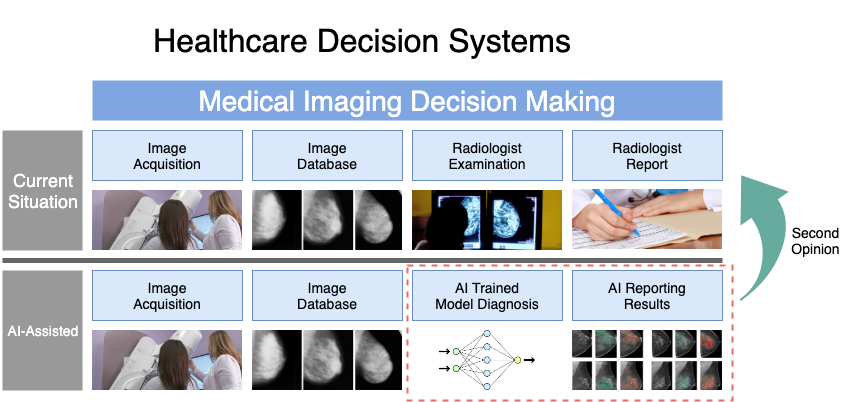
\includegraphics[width = \columnwidth]{./figures/fig001}
\source{\textcite{MIPDMSAI2019}.}
\end{figure}

We propose and measure a second opinion in regard to the current \textit{RR} situation~\cite{https://doi.org/10.13140/rg.2.2.16566.14403/1}.
The second opinion will take advantage of our AI trained models (CDSS), as well as it reporting results.
To measure efficiency and efficacy of our CDSS we will use a set of scales. The scales are: (1) NASA-TLX; (2) SUS; and (3) DOTS.

\vspace{10mm}

\end{block}

\end{column}

\end{columns}

\begin{columns}[t]

\begin{column}{0.945\textwidth}

\begin{block}{FRAMEWORK}

The next Figures~\ref{fig:fig002}, \ref{fig:fig003} e \ref{fig:fig004} are samples of our working CDSS:

\begin{column}[T]{0.33\textwidth}
\begin{figure}[!htb]
\centering
\caption{UI CDSS overview showing a patient's US image.}
\label{fig:fig002}
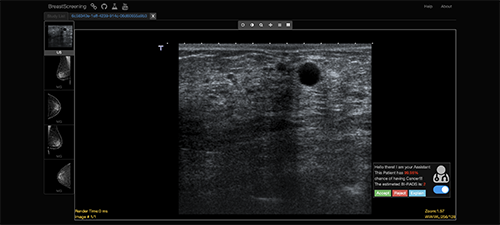
\includegraphics[width = 0.75\columnwidth]{./figures/fig002}
\end{figure}
\end{column}
{\color{PosterBars}\vrule width 1.5pt}
\begin{column}[T]{0.33\textwidth}
\begin{figure}[!htb]
\centering
\caption{The CDSS oracle and interaction.}
\label{fig:fig003}
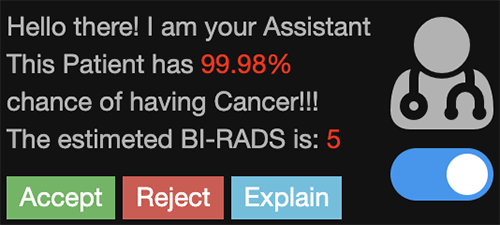
\includegraphics[width = 0.75\columnwidth]{./figures/fig003}
\end{figure}
\end{column}
{\color{PosterBars}\vrule width 1.5pt}
\begin{column}[T]{0.33\textwidth}
\begin{figure}[!htb]
\centering
\caption{Result of the eXplainability (XAI) techniques.}
\label{fig:fig004}

\includegraphics[width = 0.75\columnwidth]{./figures/fig004}
\end{figure}
\end{column}

\end{block}

\end{column}

\end{columns}

\hfill

\begin{columns}[t]

\begin{column}{0.45\textwidth}

\begin{block}{FUTURE WORK AND CONCLUSIONS}

Our work is a first attempt to test the potential of Radiomics in a real-world clinical scenario.
More than answering our research questions it opens a number of new avenues for further investigation.
This research leverages on previous work implementing DL for active breast lesion detection.
However, integrating the CDSS on a pipeline requires a lot of engineering work.
For effective clinical application, our work requires a proper clinical trial procedure which is out of the scope of this poster.
Ultimately, we believe there is significant room for future research - to which this work is an important but only initial step - and we hope to see further exploration.

\end{block}

\vspace{10mm}

\begin{block}{ACKNOWLEDGEMENTS}
\footnotesize
Support received for the development of this work and participation in this event:
\vfill

\includegraphics[height = 29mm]{./logos/logo005}
\hspace*{5mm}

\includegraphics[height = 29mm]{./logos/logo006}
\hspace*{5mm}

\includegraphics[height = 29mm]{./logos/logo007}
\hspace*{5mm}

\includegraphics[height = 29mm]{./logos/logo008}
\hspace*{5mm}

\includegraphics[height = 29mm]{./logos/logo009}
\end{block}

\end{column}

\begin{column}{0.45\textwidth}

\begin{block}{REFERENCES}
\printbibliography[heading = none]
\end{block}

\end{column}

\end{columns}

\end{frame}

\end{document}
